\section{Experiments and Analysis}
\label{sec.exp}

\begin{figure}[t]
    \centering
    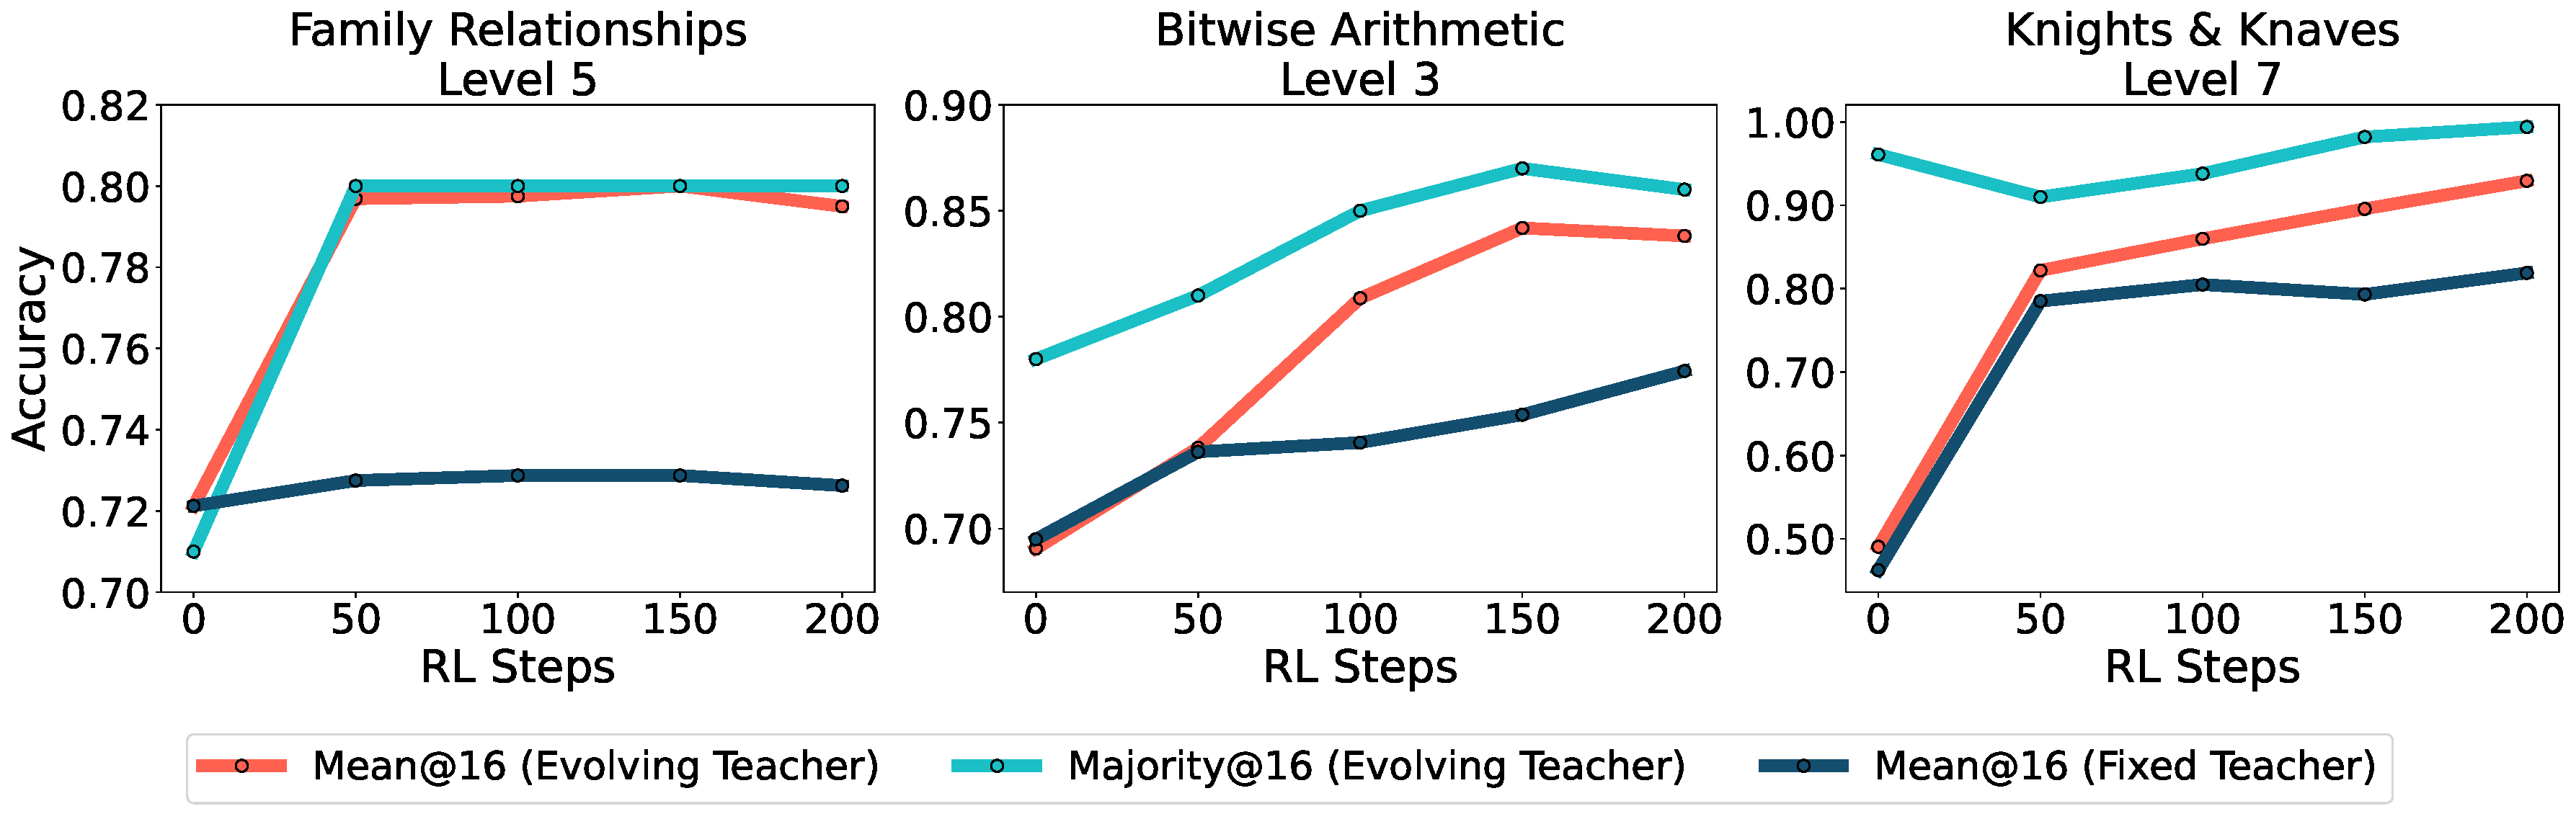
\includegraphics[width=0.95\linewidth]{Figures/reasoning_gym/reasoning-gym-main-plot.pdf}
    \caption{\footnotesize (\textbf{\algo{} improves both performance and quality of generated labels during training.}) We investigate self-training under controlled settings on synthetic reasoning tasks from Reasoning Gym. Remarkably, \algo{} improves not only the mean accuracy, but the majority voting accuracy as well, which is the source of our training supervision. Improvement in the quality of training signal drives further improvement in performance, as \algo{} outperforms its variant employing the majority votes from a fixed teacher as proxy labels.}
    \label{fig:reasoning-gym-main-plot}
\end{figure}

In this section, we present the results of our empirical study. Our primary aim is to answer the two following research questions: \textbf{(1)} \textbf{Can \algo{} improve an LLMs' reasoning abilities beyond the base model's capabilities}, 
in terms of both the quality of training reward signal and performance on downstream tasks? Specifically, since simply performing majority voting on the base model can improve performance compared to individual generations, can we improve the quality of the majority votes (which acts as the verifier for \algo{}) in addition to pass@1 performance compared to the base model via \algo{}?  \textbf{(2)} If \algo{} can go beyond the base model, \textbf{can this improvement be sustained indefinitely?} We systematically design experiments to answer these questions below.


\subsection{Can \algo{} go beyond the base model's capabilities?} \label{sec:question_1}

There are two potential axes of improvements over the base model for \algo{} that can be studied: (1) the improvement in accuracy over held-out prompts, and (2) the improvement in the quality of generated labels themselves during the training procedure. Unlike previous works~\citep{huang-etal-2023-large,prasad2024selfconsistencypreferenceoptimization} that distill the majority voting decision of a fixed policy (typically the base model) into the current model, we want to study \textbf{whether the quality of the majority votes of the evolving policy improves} as a result of self-improvement. 

\begin{figure}[t]
    \centering
    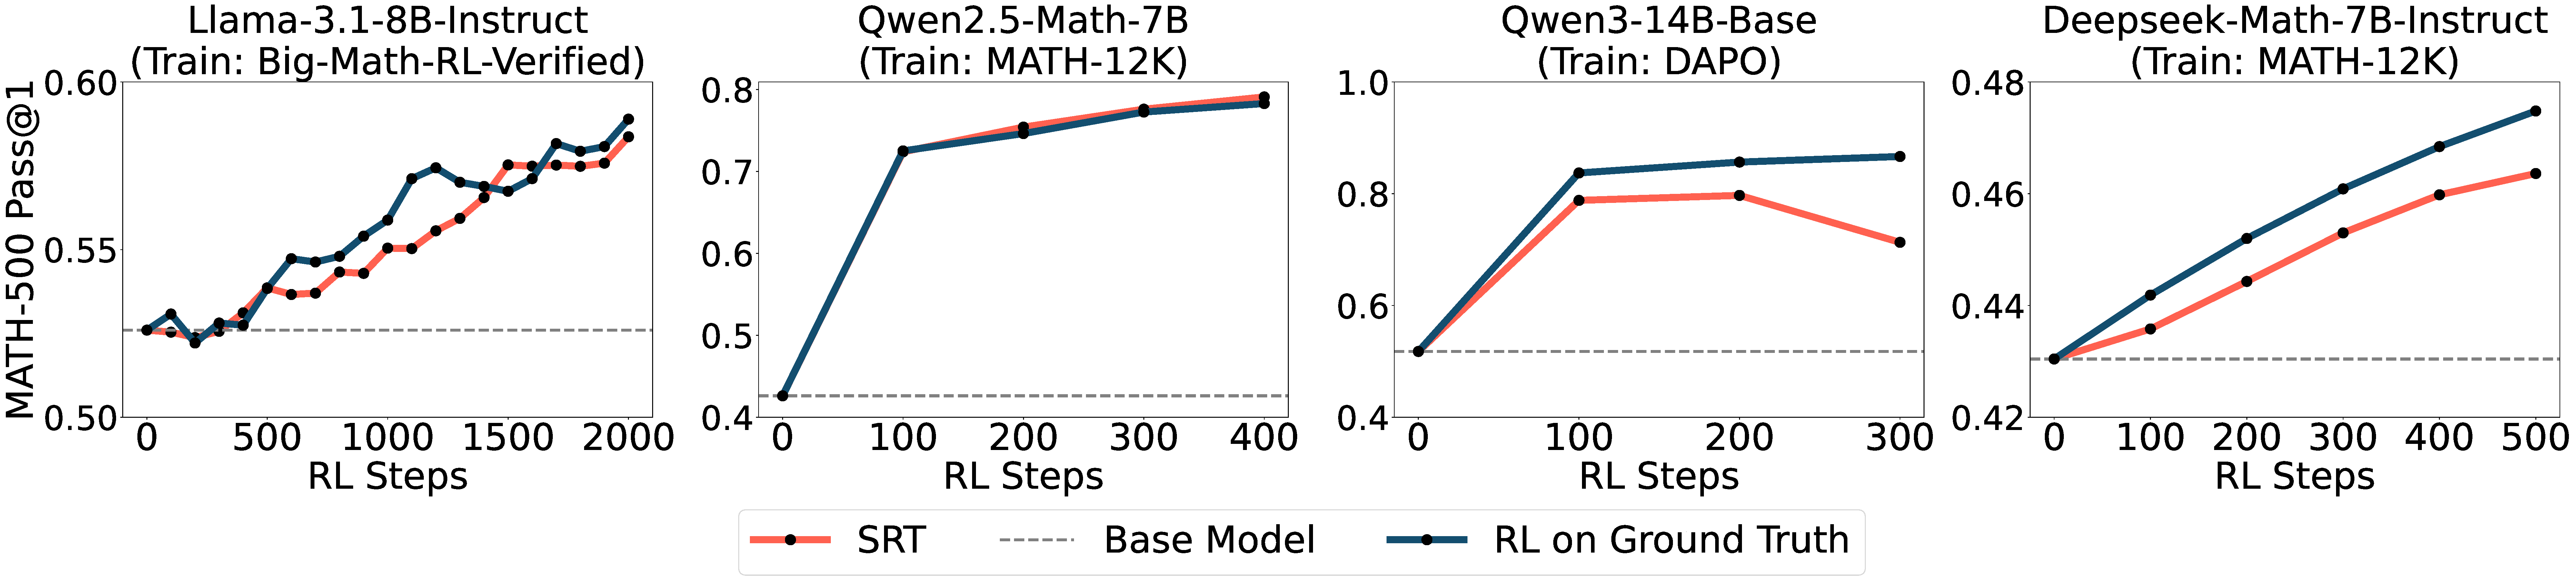
\includegraphics[width=0.99\linewidth]{Figures/section_4.1/all_model_average_accuracy_math_500.pdf}
    \caption{\footnotesize \textbf{(Evaluating \algo{} on real-world math problems.)} Comparison between \algo{} and RL with ground truth across different base models and training datasets. Following~\citep{Oertell2024Heuristics}, all models are trained using RLOO (for experiments with GRPO, see Figure~\ref{fig:grpo_vs_rloo_all_test_datasets}) and tested using average pass@1 accuracy on MATH-500. \algo{} achieves comparable performance to that of ground-truth training across different base models. For training curves using more combinations of (train, test) dataset pairs, refer to Appendix~\ref{app:qwen2.5_math_7b_full_results} and~\ref{app:qwen3_full_results}.}
    \label{fig:all_model_average_accuracy_math_500}
\end{figure}

\begin{figure}[t]
    \centering
    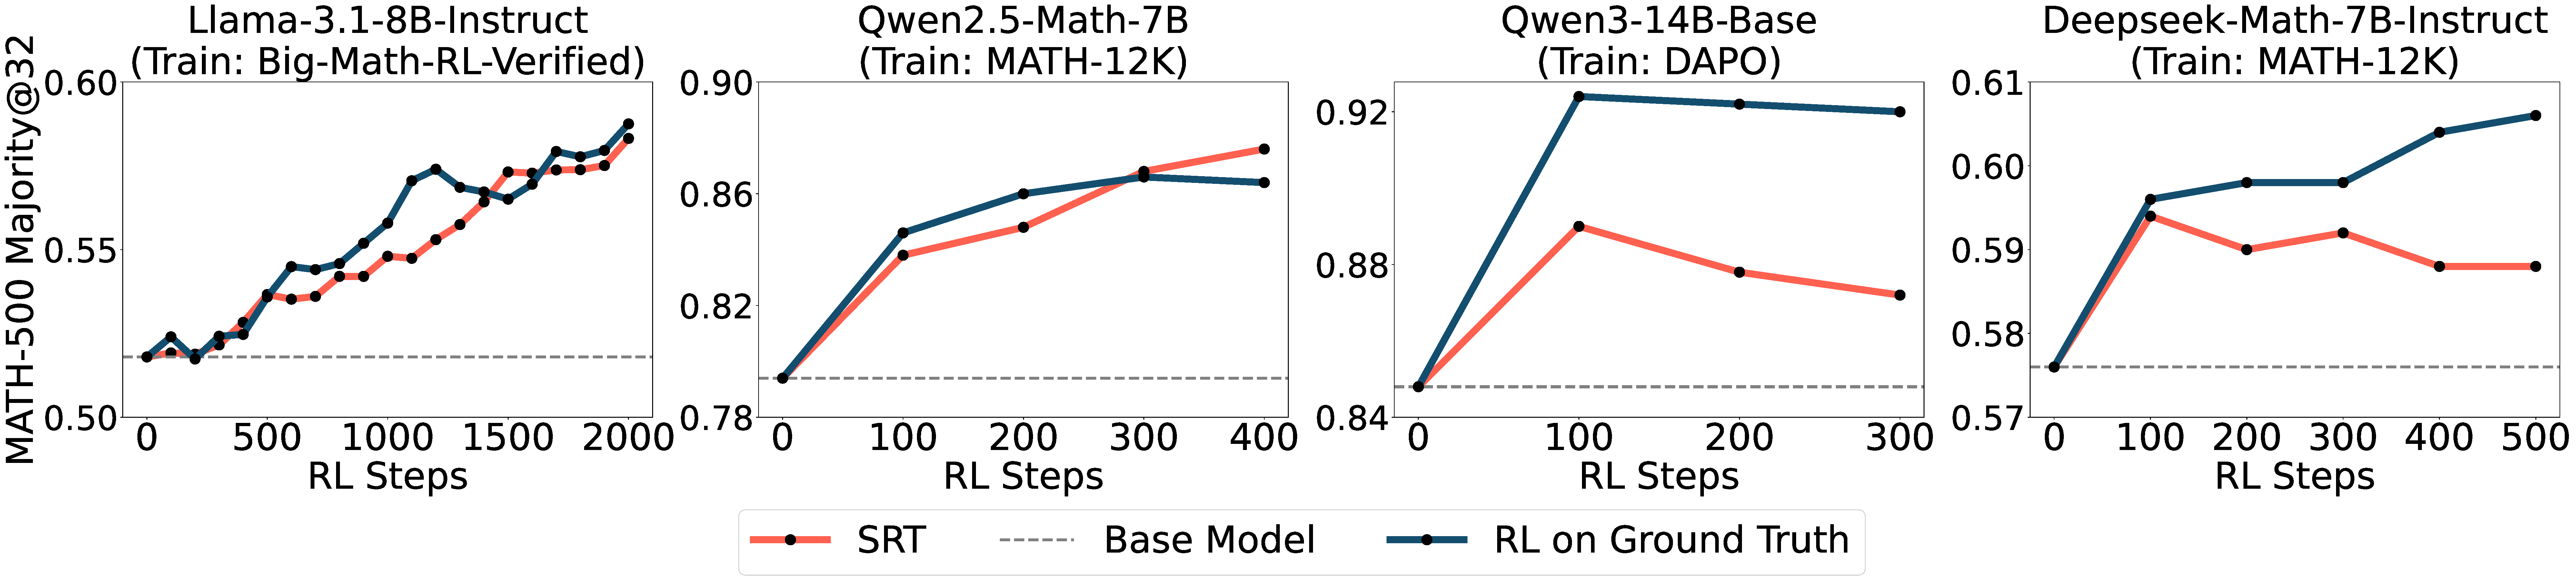
\includegraphics[width=0.99\linewidth]{Figures/appendix/all_model_majority_accuracy_math_500.pdf}
    \caption{\footnotesize \textbf{(Majority@32 accuracy comparison between \algo{} and RL with ground truth)} We compare the majority@32 accuracy, as opposed to average accuracy shown in Figure~\ref{fig:all_model_average_accuracy_math_500}. \textbf{Note that for Llama-3.1-8B-Instruct, we use the official model card evaluation temperature of 0, hence majority@32 is the same as average@32 accuracy.} \algo{} shows improvement in the quality of the majority votes themselves, which distinguishes our algorithm from that of learning from a fixed teacher's majority votes.}
    \label{fig:all_model_majority_voting_accuracy_math_500}
\end{figure}


\paragraph{Experiments on synthetic reasoning tasks.} 
Complex reasoning tasks like math require domain-specific pre-training/midtraining for online RL to be effective~\citep{wu2025miragemethodmodeltaskalignment,gandhi2025cognitivebehaviorsenableselfimproving}; it is also more difficult to control the difficulty of the individual tasks that the model sees during training. Therefore, we first study this question using synthetic reasoning tasks from REASONING GYM~\citep{stojanovski2025reasoninggymreasoningenvironments}, a collection of over 100 reasoning environments for reinforcement learning with verifiable rewards. These tasks can also be generated with adjustable difficulty, making it a suitable test-bed for our work. Concretely, we use 3 tasks from Reasoning Gym: \textbf{(1)} \textbf{Family Relationships}, a logic puzzle involving a group of individuals connected via different relationships, and the model has to reason about the relationship between two individuals within this group, \textbf{(2)} \textbf{Bitwise Arithmetic}, a task for testing models' understanding of Bitwise Arithmetic operations, and \textbf{(3)} \textbf{Knights \& Knaves}, a logic puzzle involving characters who always either tell the truth (knights) or always lie (knaves), and the challenge is to deduce who is who based on their statements. Appendix~\ref{app:reasoning_gym_example_tasks} shows example prompts from each of these tasks. We use a Qwen-3-4B-Base~\citep{yang2025qwen3technicalreport} model for all our reasoning gym experiments.

Since our goal is to study whether \algo{} can improve performance on top of a reasonably strong base model, following the setting of~\citet{lee2025selfimprovingtransformersovercomeeasytohard}, we first train the base model with GRPO using ground truth labels on the easiest difficulty setting. This is used to teach the base model proper formatting rules and how to solve the basic task before we train using \algo{} on the next level of difficulty without ground-truth labels. The detailed training settings can be found in Appendix~\ref{app:training_hparam_details}.

\paragraph{Results.} Figure \ref{fig:reasoning-gym-main-plot} shows our main results: \algo{} using the current policy as the label generator improves both avg@16 and majority vote@16 accuracy on all 3 reasoning gym tasks. Since we derive our training signal from the majority votes of the current policy evolving with every RL step --- this demonstrates that self-improvement using \algo{} can progressively improve the quality of the pseudo-labels as well. Note that this would not be possible in prior works~\citep{prasad2024selfconsistencypreferenceoptimization,huang-etal-2023-large} which distills the majority votes of a \emph{fixed teacher} policy throughout one round of training. We expect the improvement in the \emph{evolving teacher} policy to result in further performance gain. To validate this, we compare \algo{} with a variant of the same algorithm where we use the majority votes of the fixed starting policy instead of the evolving current policy as pseudo-labels. Figure \ref{fig:reasoning-gym-main-plot} shows their comparison: in Family Relationships and Bitwise Arithmetic, we see larger gains in majority voting performance, and likewise \algo{} outperforms its fixed teacher variant substantially, by 10\% for Bitwise Arighmatics, 8\% in Family Relationship, and 6\% in Knights and Knaves. On Knights \& Knaves, the starting policy already has >90\% majority voting accuracy, and we see the difference between the evolving teacher and fixed teacher variants of \algo{} to be smaller here. Furthermore, these performance gains cannot be explained by learning to format properly: since the model was trained on an easier difficulty level, it can already format its responses correctly in most cases (Appendix~\ref{app:parsability_metrics}), and we see performance climbing after saturation in model's format correctness. Overall, on the synthetic reasoning tasks, \textbf{\algo{} clearly pushes the model beyond its starting capabilities}, showing the promise of self-improvement even from this basic recipe for self-supervision.

We show a summary of our empirical findings using different base models and training datasets in Figures~\ref{fig:all_model_average_accuracy_math_500} and~\ref{fig:all_model_majority_voting_accuracy_math_500} (for training curves using more combinations of (train, test) dataset pairs, refer to Appendix~\ref{app:qwen2.5_math_7b_full_results} and~\ref{app:qwen3_full_results}). On all instances, \algo{} improves both avg@16 and majority vote@16 accuracies on heldout MATH-500 prompts, and performs on par with regular RL training with ground truth verification. More impressively, the observations hold for base models like Llama-3.1-8B-Instruct, which is known to be particularly difficult for RL training on reasoning tasks~\citep{gandhi2025cognitivebehaviorsenableselfimproving}, improving its average accuracy from 52.6\% to nearly 60\%.

We also compare \algo{} with its offline variants: SFT on the majority vote~\citep{huang-etal-2023-large}, DPO and ScPO~\citep{prasad2024selfconsistencypreferenceoptimization} employing contrastive learning between the majority vote and non-majority vote answer in Table~\ref{tab:baseline_comparison}. We observe that \algo{} retains better performance compared to its offline variants distilling the majority vote decisions of the base policy, \textbf{showing the benefit of self-improvement in the label-generating policy}. For more details about the baselines, including choice of hyperparameters and performance on additional test datasets, refer to Appendix~\ref{app:baseline_details}.

\begin{table}[h!]
    \centering

    \caption{\footnotesize \textbf{(Peak Performance)} We compare \algo{} against various baselines using a Qwen2.5-Math-7B model. Reported numbers are peak mean@32 accuracy, averaged over 3 heldout datasets: AIME 2024, AIME 2025, AMC. We find that \algo{} generally retains better performance compared to baseline methods distilling the majority voting decisions of the fixed teacher policy into the current model.}
    
    \resizebox{0.75\textwidth}{!}{%
        \begin{tabular}{c|ccccc|c}
        \toprule
            Train Data & Base Model & SFT & DPO & ScPO & \algo{}  & RL on Ground Truth \\
        \midrule
        MATH-12K & 0.15 & 0.18 & 0.23 & 0.20 & 0.32 & 0.33 \\
        DAPO & 0.15 & 0.18 & 0.21 & 0.20 & 0.31 & 0.36\\
        \bottomrule
        \end{tabular}
    }
    \vspace{10pt}
    \label{tab:baseline_comparison}
\end{table}


\begin{AIbox}{Takeaway 1: \algo{} can improve reasoning capabilities beyond the base model}
On both synthetic and real reasoning tasks, \algo{} improves average and majority voting accuracies, showing ability gains beyond the base model. Specially, improvement in majority voting accuracy also signifies improvement in the quality of generated self-supervision during training, demonstrating the importance of training the ``verifier'' in addition to just training the policy. Overall, our simple recipe shows a promising path forward to self-improvement. 
\end{AIbox}
\vspace{-0.1cm}

\subsection{Can Self-Improvement from \algo{} be Sustained Indefinitely?} \label{sec:question_2}

Given the strong performance of \algo{} in various reasoning tasks and model architectures, an important question is whether self-training can be maintained over extended iterations. Similar to the prior section, we first test \algo{} on synthetic tasks with controllable difficulty to rigorously study its properties, and then test the resulting insights on real-world reasoning domains.

\begin{figure}[h]
    \centering
    \vspace{-0.2cm}
    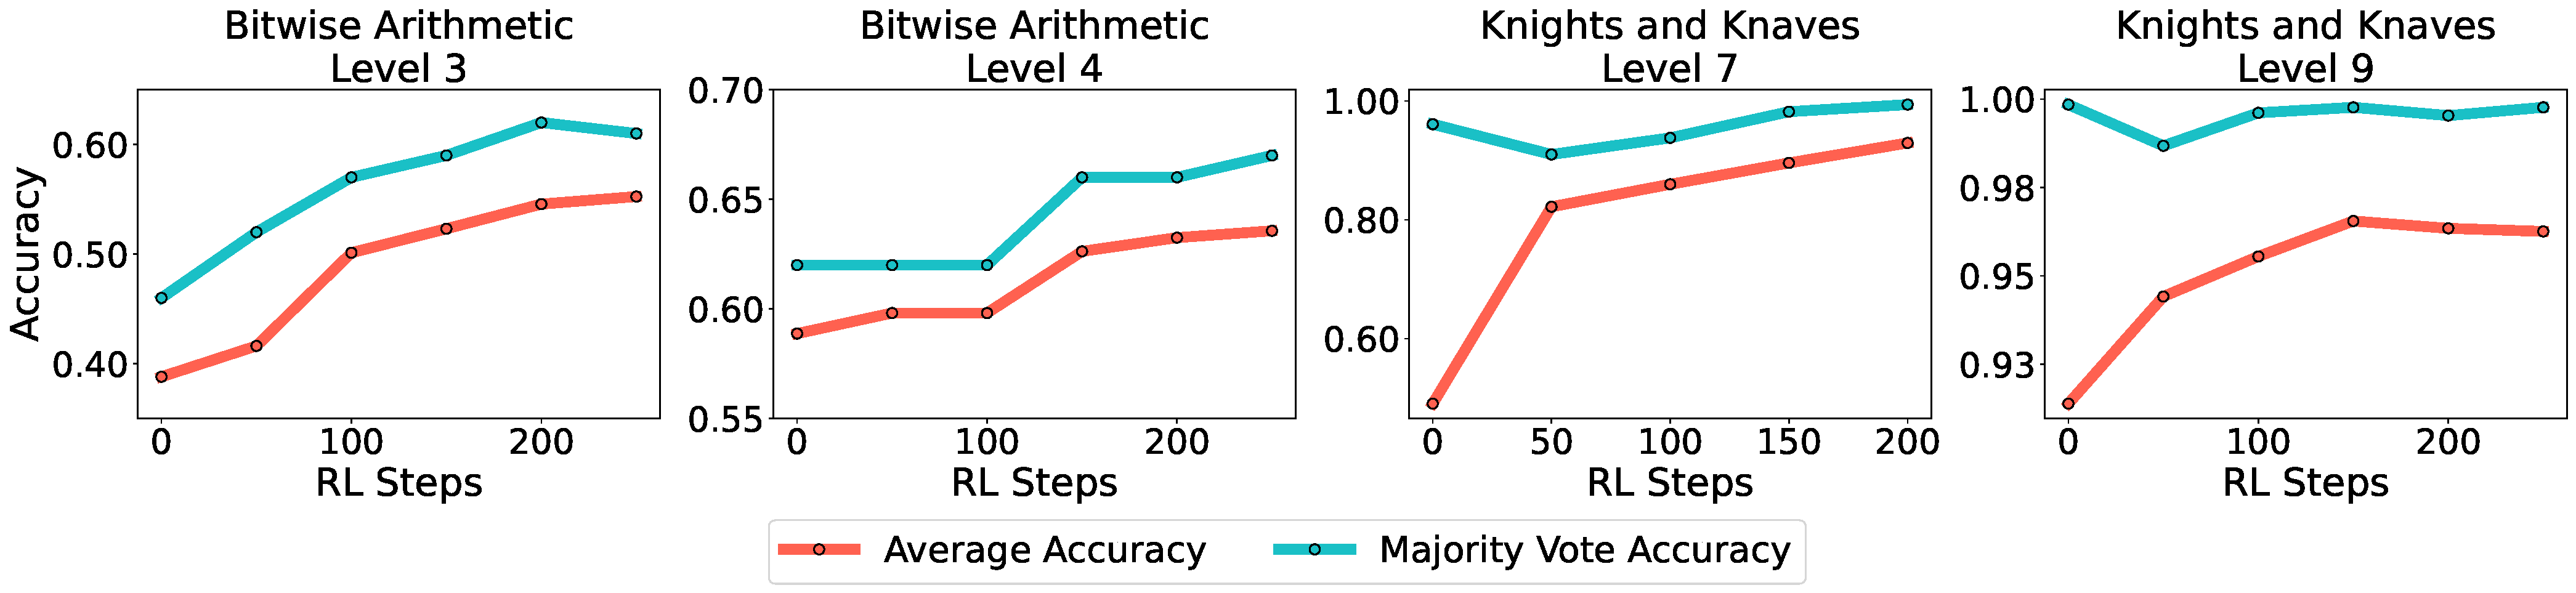
\includegraphics[width=0.99\linewidth]{Figures/reasoning_gym/multistep-climbing.pdf}
    \caption{\footnotesize \textbf{(Multi-level climbing on Reasoning Gym using curriculum)} The Qwen3-4B-Base model can climb on progressively more difficult tasks without ground truth labels via a simple curriculum strategy --- where we train an earlier level's final checkpoint with \algo{} on the next difficulty level. This approach also seems to improve both average and majority voting accuracy on each level.}
    \label{fig:multi-step-climbing}
    \vspace{-0.4cm}
\end{figure}

\paragraph{Multi-level self-improvement on synthetic tasks using curriculum.} Since Reasoning Gym provides a built-in way to control the difficulty of generated tasks, we first investigate whether self-training on an easier set of tasks can produce a model capable of self-improvement on progressively harder levels of difficulty. To do so, we choose 2 Reasoning Gym tasks: Bitwise Arithmetic and Knights \& Knaves. Similar to our previous setting, we first train using RL on ground truth labels on the easiest level of difficulty, then progressively train on harder levels without ground truth labels (i.e., \algo{} on level 5 starts with the checkpoint obtained from \algo{} on level 4, and so on). For more details, refer to Appendix~\ref{app:training_hparam_details}. 

Figure \ref{fig:multi-step-climbing} shows our primary results: in this controlled setting, \algo{} is able to maintain self-improvement on progressively harder difficulties. In particular, \algo{} can show reasonable improvement in Bitwise Arithmetic Level 4 after being initialized on Level 2 with ground-truth training, and also progressively climb to near 100\% accuracy on Knights \& Knave Level 9 after being trained with ground-truth on Level 2 only (intermediate levels are trained with \algo{}). In synthetic reasoning tasks where we have a knob for controlling the difficulty of training problems, even the simple curriculum of progressively training on more difficult problems with self-supervision can maintain improvement across multiple difficulty levels.   

\begin{figure}[h]
    \centering
    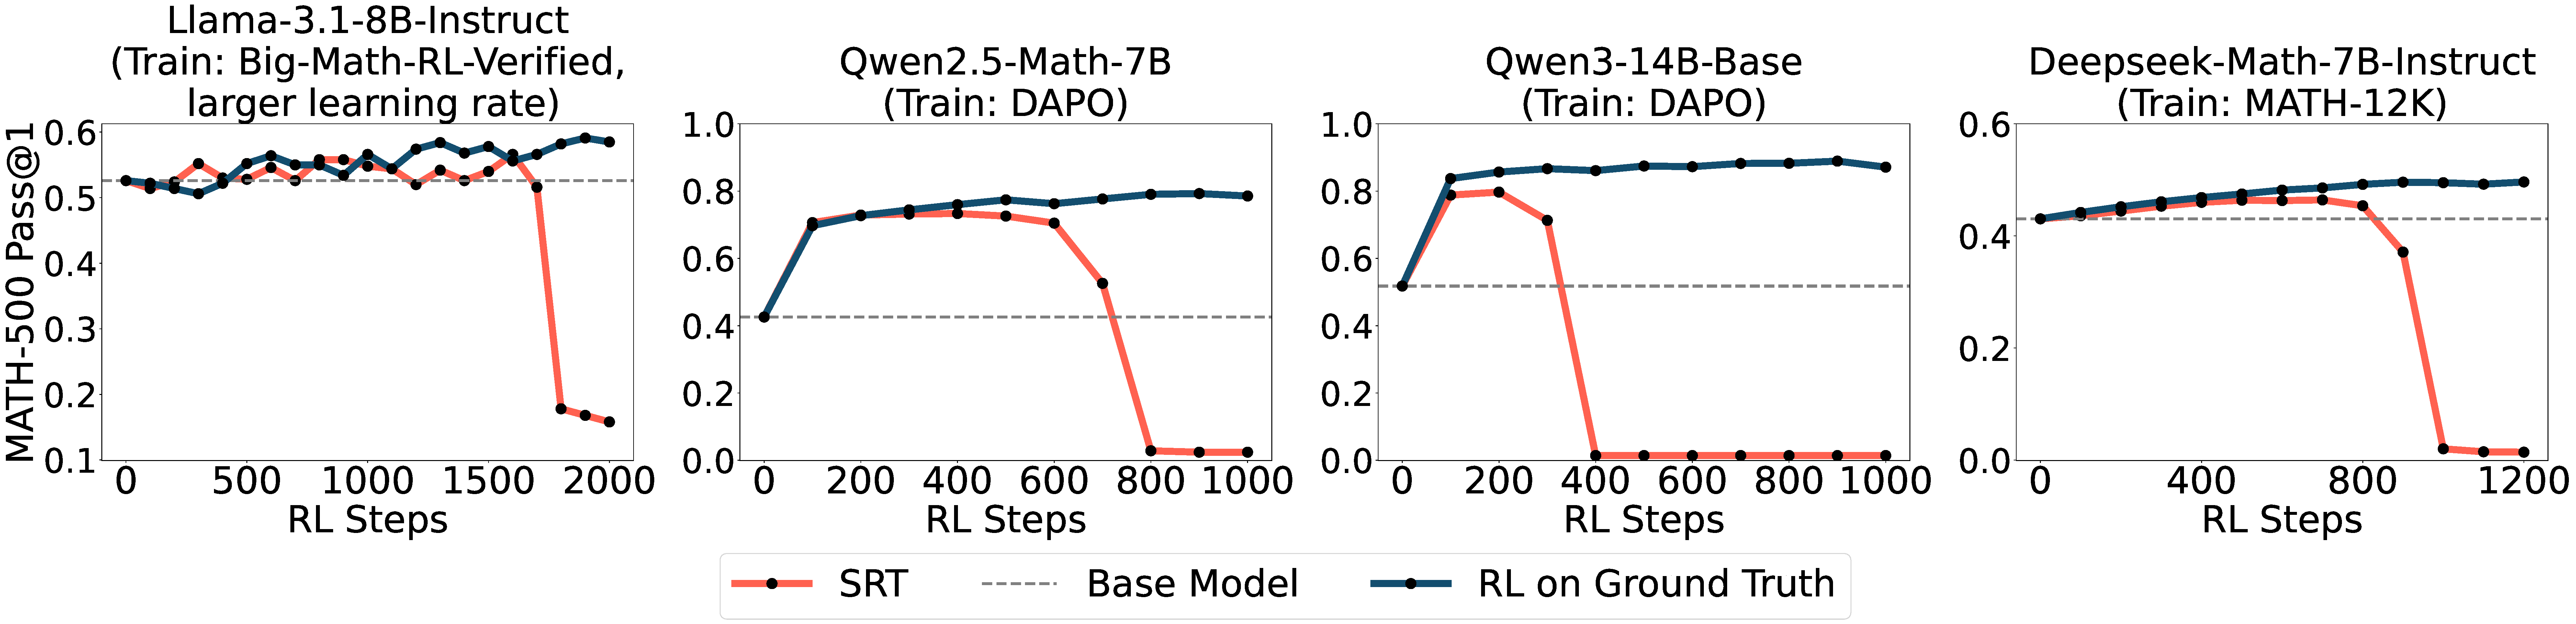
\includegraphics[width=0.99\linewidth]{Figures/section_4.2/demonstrating_model_collapse.pdf}
    \caption{\footnotesize \textbf{(Extended self-training leads to model collapse)} Inspired by multi-level improvement on reasoning gym tasks, we take four LLMs with strong math abilities from pretraining, and train them with \algo{} for an extended period of time. \algo{} improves performance at first, but then demonstrates complete model collapse on all 4 base models. (Note: on Llama-3.1-8B-Instruct, the learning rate used in Figures~\ref{fig:all_model_average_accuracy_math_500} and ~\ref{fig:all_model_majority_voting_accuracy_math_500}, $10^{-7}$, does not lead to model collapse within our training budget, but $3 \times 10^{-7}$, a slightly higher learning rate does --- we hypothesize that with an extended training run, even $10^{-7}$ would lead to model collapse. For more details on the effect of hyperparameters on model collapse, refer to Figure~\ref{fig:training_choice_summary}.)}
    \label{fig:demonstrating_model_collapse}
    \vspace{-0.3cm}
\end{figure}

\paragraph{Extended \algo{}-training on math problems.} Next, we test whether our insights from synthetic tasks also extend to real-world math problems. Specifically, we take take the same 4 base models as in the previous section, and train them on a difficult math dataset through an extended number of iterations using \algo{}. Figure~\ref{fig:demonstrating_model_collapse} demonstrates our surprising finding: while \algo{} initially increases the base model's performance at a comparable rate with ground-truth RL training, extended training using \algo{} leads to sudden performance collapse. \textbf{We observe performance collapse or degradation from extended \algo{}-training across all models and training datasets,} and record these in detail in Appendix~\ref{app:qwen2.5_math_7b_full_results} and~\ref{app:qwen3_full_results}. Given that this surprising phenomenon deserves more investigation, we study it in more detail next.

\paragraph{What happens after \algo{} peaks in performance?} 

To develop a clearer understanding of the underlying reasons for this phenomenon, in this section we investigate this \algo{}-induced model collapse closely.

We plot the training statistics of the \algo{} objective (Eqn. \ref{eqn:self-reward}) in Figure \ref{fig:dynamics_of_model_collapse}. The observed performance collapse closely coincides with a sudden increase in the \algo{} self-reward objective, implying that the optimization procedure has, in fact, maximally optimized the training objective (self-consistency majority voting), despite a decline in \textit{actual} output correctness. On the same figure, we further report the token-level average Kullback–Leibler divergence between the model under \algo{} training and the base model. We observe a sharp increase in KL divergence at the exact point when performance begins to deteriorate, indicating that the generative distribution of the model has substantially diverged from the original model.

\begin{figure}[t!]
    \centering
    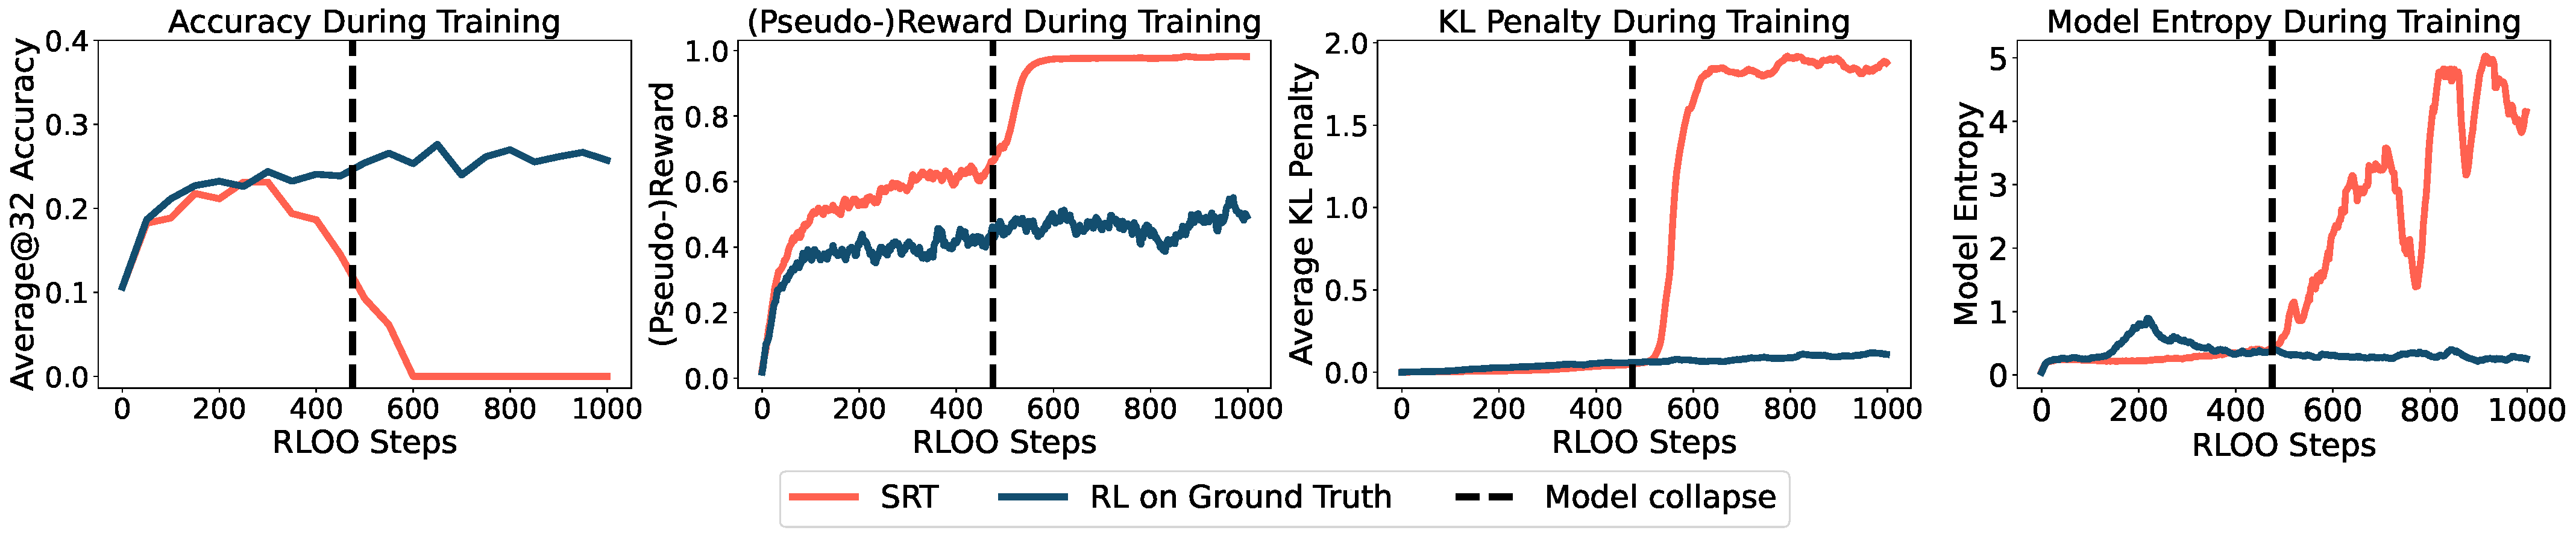
\includegraphics[width=0.99\linewidth]{Figures/section_4.2/dynamics_of_model_collapse_during_srt.pdf}
    \caption{\footnotesize \textbf{(Self-Training Dynamics)} Extended training via \algo{} can lead to reward hacking, as demonstrated by the sudden hike in KL penalty and training (psuedo-)reward, but collapse of accuracy on the held-out test sets.}
    \vspace{-0.3cm}
    \label{fig:dynamics_of_model_collapse}
\end{figure}

These findings strongly suggest the occurrence of \textbf{reward hacking}---the model has learned to produce consistent responses in order to optimize its self-assigned reward, irrespective of their true correctness. Indeed, manual analysis of the model outputs (examples provided in Appnedix \ref{app:reward_hacking_examples}) confirms this hypothesis: \textbf{after collapse, the model outputs a very high entropy, essentially random, set of tokens followed by the same ``template'' final answer} (for example, \texttt{\string\boxed\{1\}}) that is nearly independent of the input prompt).
In other words, the initially strong correlation between the \algo{} objective and correctness is ultimately compromised, becoming no longer a reliable proxy signal. 
This behavior is also related to the well-known simplicity bias in neural networks~\citep{depalma2019randomdeepneuralnetworks,vallepérez2019deeplearninggeneralizesparameterfunction,mingard2020neuralnetworksprioribiased,Mingard2025Deep}, as well as the Occam's razor, where neural networks tend to find the simplest solution that generalizes to the observed signal --- in this case this leads to the same final template answer for all prompts.

\begin{figure}[h]
    \centering
    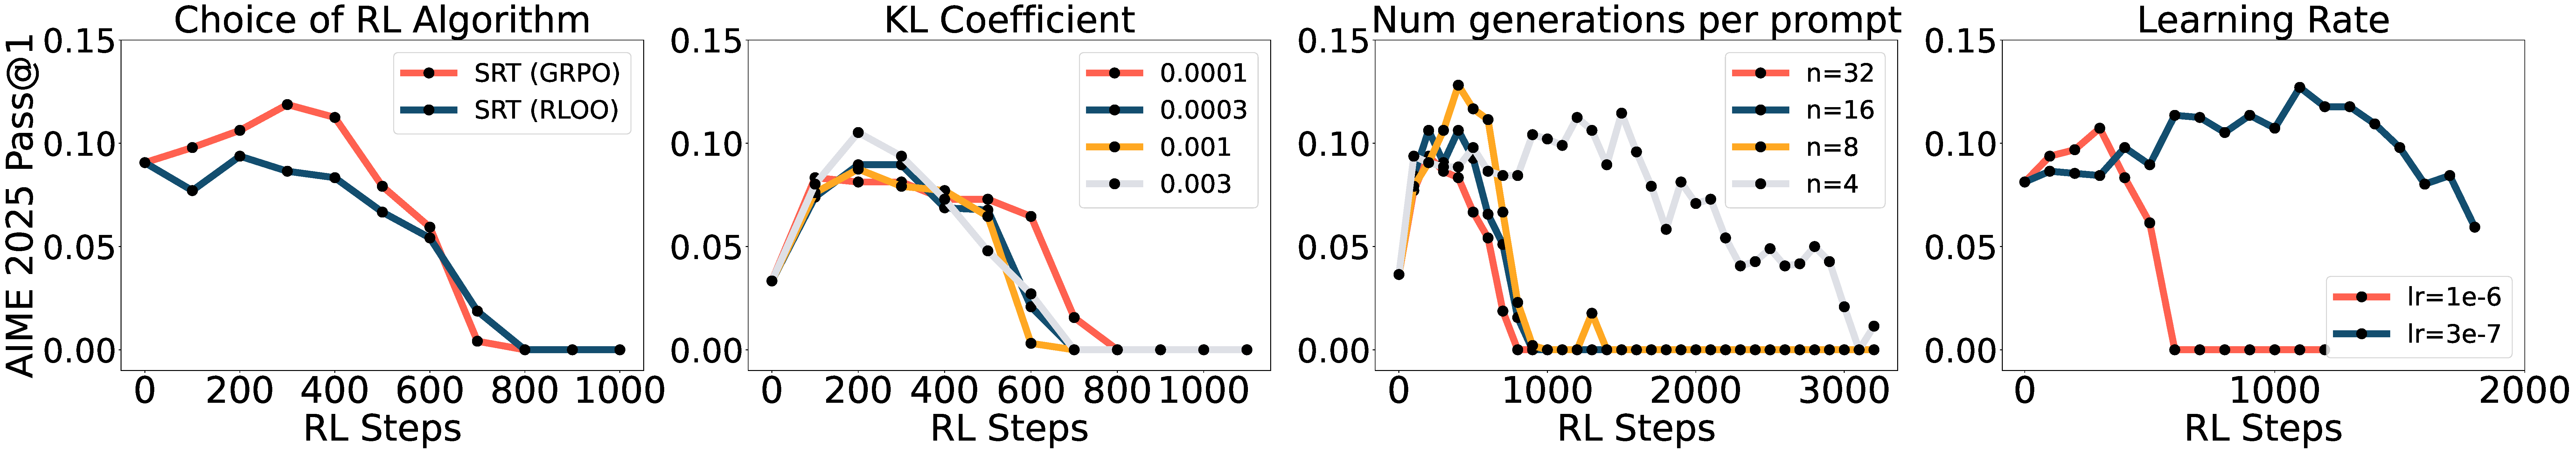
\includegraphics[width=0.99\linewidth]{Figures/section_4.2/training_choice_summary.pdf}
    \caption{\footnotesize \textbf{(Sweep over training configurations)} We vary the training settings for \algo{} from the default ones described in Appendix~\ref{app:training_hparam_details} and record the observations. All experiments are run using Qwen2.5-Math-7B on DAPO. Evaluations are done using AIME 2025, but other datasets show similar behavior. In summary, choice of RL algorithm between GRPO and RLOO, and different KL coefficients do not affect model collapse significantly. Lowering learning rate slows down model collapse as expected. Finally, reducing number of generations injects noise into the majority vote, surprisingly resulting in a slow down of model collapse.}
    \label{fig:training_choice_summary}
\end{figure}

\paragraph{Additional experiments and ablations.}
We have run additional experiments and ablations to study the behavior of self-training under different training scenarios. Figure~\ref{fig:training_choice_summary} shows our main findings: \textbf{(1)} choice of RL algorithm (GRPO vs RLOO) does not affect the final outcome of \algo{}-training, \textbf{(2)} increasing KL coefficient to incentivize the model to stay close to the base policy also does not mitigate reward hacking, as the training signal from the reward hacked solution is too strong, \textbf{(3)} decreasing learning rate seems to delay model collapse but not eliminate it, and we hypothesize that prolonged training with lower learning rates would still result in complete model collapse, and \textbf{(4)} surprisingly, reducing the number of generations per prompt injects noise into the training signal, which delays quick model collapse by exploiting the majority voting answer. Additional experiments related to \algo{} training, including training curves on all test datasets and effect of tuning additional hyperparameters like entropy coefficient, can be found in Appendix~\ref{app:additional_experimental_results} and~\ref{app:detail_on_hp_ablations}. We also investigated various mitigation strategies for \algo{}-induced model collapse, including early stopping, curriculum learning, and employing a fixed teacher to generate labels -- refer to Appendix~\ref{sec5.mitigation} for our findings.


\begin{AIbox}{Takeaway 2: Self-Training benefits may not extend indefinitely}
The question of whether self-training can be extended indefinitely has mixed results: while under controllable difficulty, \algo{} can keep improving beyond the base model on progressively more difficult tasks, training on real-world math problems demonstrate the phenomenon of reward hacking --- sustained self-improvement requires developing additional regularization measures to be effective.
\end{AIbox}
\vspace{-0.1cm}













    
    









